\documentclass[a4paper,12pt]{article}

\usepackage[T1]{fontenc}
\usepackage{graphicx} % for including graphics
\usepackage{longtable} % for tables that span multiple pages (if needed)
\usepackage[a4paper, top=2cm, bottom=2cm, left=2cm, right=1.8cm]{geometry}
\usepackage{pgfplots} % For plotting graphs
\usepackage[utf8]{inputenc}
\usepackage{listings}
\usepackage[serbian]{babel}

\definecolor{codegreen}{rgb}{0,0.6,0}
\definecolor{codegray}{rgb}{0.5,0.5,0.5}
\definecolor{codeblue}{rgb}{0.05,0.27,0.72}
\definecolor{backcolour}{rgb}{0.95,0.95,0.92}

\lstdefinestyle{mystyle}{
    backgroundcolor=\color{backcolour},   
    commentstyle=\color{codegreen},
    keywordstyle=\color{magenta},
    numberstyle=\footnotesize\color{codegray},
    stringstyle=\color{codeblue},
    basicstyle=\ttfamily\footnotesize,
    breakatwhitespace=false,         
    breaklines=true,                 
    captionpos=b,                    
    keepspaces=true,                 
    numbers=left,                    
    numbersep=5pt,                  
    showspaces=false,                
    showstringspaces=false,
    showtabs=false,                  
    tabsize=2
}



% Define your style
\lstdefinestyle{pisaniCstyle}{
    keywordstyle=\color{magenta}\ttfamily,
    basicstyle=\ttfamily\normalsize,
    keepspaces=true
}

% Adjust vertical space before and after code blocks
\lstset{
    aboveskip=10pt,    % Vertical space before code block
    belowskip=10pt     % Vertical space after code block
}

\title{OBARADA I ANALIZA MEDICINSKIH SLIKA \\ Smeinarski rad: Brojanje kvadrata}
\author{Ismar Osmanović / Lejla Zahirović}
\date{\today}

\begin{document}
\begin{center}
\thispagestyle{empty}
\large{UNIVERZITET U TUZLI \\ FAKULTET ELEKTROTEHNIKE}

\noindent\rule[7pt]{\linewidth}{0.4pt}


  
\includegraphics[width=0.7\linewidth]{fet_logo.png}
\vspace{3cm}\\
{\fontsize{34pt}{28pt}\selectfont SEMINARSKI RAD}\\
\large{OBARADA I ANALIZA MEDICINSKIH SLIKA}\\
\vspace{2cm}
\Huge{Tema:}\\
\Huge{Prepoznavanje kvadrata na slici}\\
\vspace{0.5cm}
\large{Ismar Osmanović / Lejla Zahirović}
\vfill

\noindent\rule[7pt]{\linewidth}{0.4pt}
\end{center}
\newpage
\thispagestyle{empty}
\tableofcontents
\newpage
\pagenumbering{arabic} 

\section{Ideja projekta}
Segmentacija slike predstavlja jedan od osnovnih problema u obradi slike. 
Zadatak našeg projekta je kreirati algoritam koji će segmentirati, a zatim i prebrojati crvene i zelene kvadate na slici.
\begin{figure}[h]
    \centering
    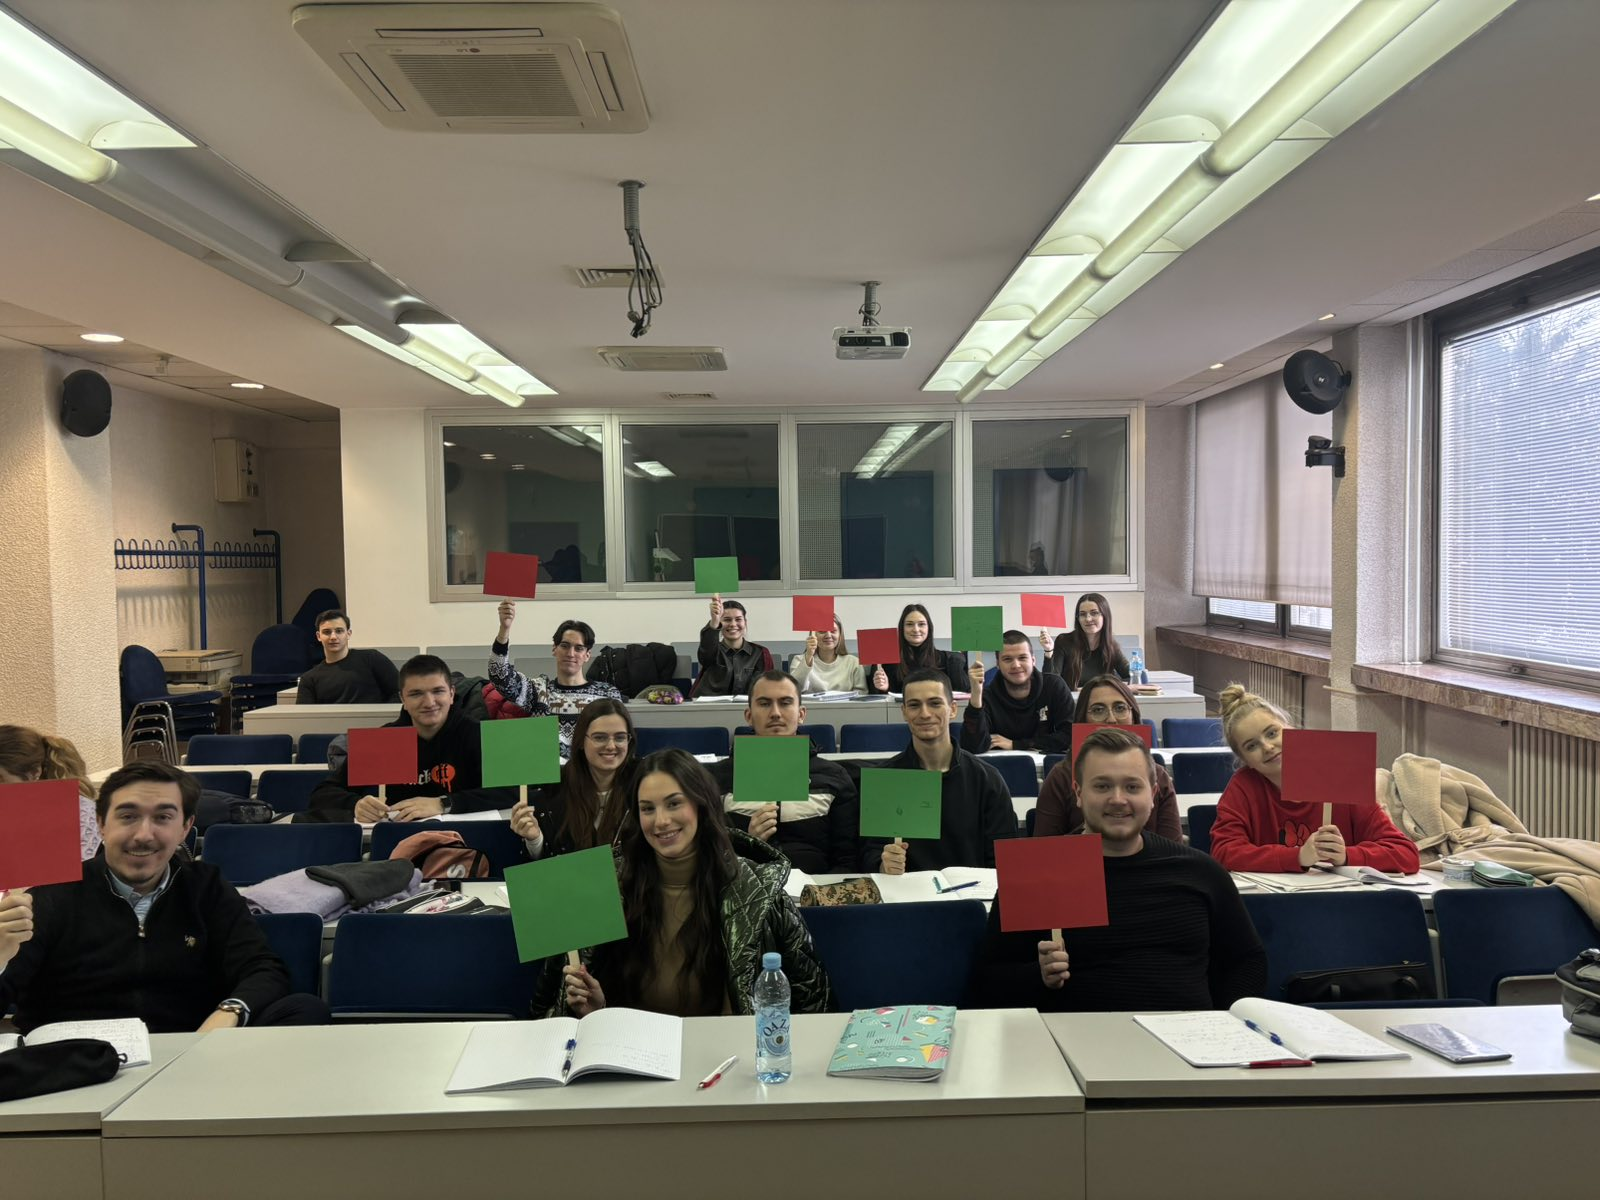
\includegraphics[width=\textwidth]{../img/studenti.jpg}
    \caption{Početna slika}
    \label{fig:example}
\end{figure}
\newpage
\section{Realizacija projekta}
\lstinputlisting[language=matlab, style=mystyle, linerange={2}]{../brojanje_kvadrata_ciz.m}
\texttt{Imread} funkcija učitava sliku iz file-a koji je specificiran pomoću njegovog imena, utvrđujući format  na osnovu sadržaja istog. 
Ako je ime file-a file sa više slika, funkcija imread učitava prvu sliku u tom file-u.
Dakle, 'img/test1.jpg' je putanja do slike koja se učitava. img je varijabla u kojoj se čuva učitana slika. 
Nakon što je slika učitana, sadržaj slike (u formi matrice piksela) biće sačuvan u varijabli “img”. Ova funkcija je dio biblioteke koju koristi MatLab.\\
\subsection{Određivanje pragova poje}
\lstinputlisting[language=matlab, style=mystyle, linerange={5}]{../brojanje_kvadrata_ciz.m}

Koristeći funkciju \texttt{rgb2hsv} slika se konvertuje iz RBG color prostora u HSV (Hue, Saturatiom, Value) color prostor. 
Dok RGB prostor koristi tri komponente (crvenu, zelenu i plavu) za reprezentaciju boja, HSV prostor koristi tri komponente:\\
\begin{itemize}
    \item Hue (boja slika kao crvena, plava),
    \item Saturation (intenzitet boje),
    \item Value(osvijetljenost boje).
\end{itemize}

Dakle, img je ulazna slika u RGB formatu, koja je pritome učitana pomoću \texttt {imread} funkcije, a “hsvImg” je promjenjljiva u kojoj će biti sačuvana slika u HSV formatu. \\

\indent Zašto je primjenjena ova konverzija, iz jednog color prostora u drugi, na ovom primjeru?\\

U opštem slučaju se u ovaj format koristi zbog svojih prednosti u obradi same slike. 
Naime, ovaj format pruža lakšu manipulaciju bojama. 
Naprimjer, H komponenta je nezavisna od svjetlosti i zasićenosti, pa je koristeći navedeni format lakše izolavati određene boje na slici, sto će kasnije biti primjenjeno, nego isključivo koristeći RGB format. 
U implementaciji koda je upravo bio zadatak pronaći piksele crvene i zelene boje na datim slikama. 
Međutim, u prvobvitnom prostoru, taj zadatak bi bio znatno otežan jer bi bilo potrebno razmatrati sve tri komponente, a u ovom slučaju smo posmatrali samo H komponentu za filtriranje crvenih tonova, kao i zelenih. 
Preostale dvije mogu biti korištene za kontrolu jačine boje i osvjetljenosti. 

\lstinputlisting[language=matlab, style=mystyle, linerange={8-11}]{../brojanje_kvadrata_ciz.m}

Ove linije koda definišu pragove za filtriranje crvene boje u HSV color prostoru. 
Konkretno, koristi se Hue (H), Saturation (S) i Value (V) komponente za postavljanje opsega boje crvene(a kasnije i zelene), tako da se mogu prepoznati pikseli koji odgovaraju toj boji u slici.

Zašto se koristi ovaj pristup?
Ovaj pristup koristi dva opsega vrednosti za Hue (H), jer crvena boja u HSV prostoru nije predstavljena sa samo jednim opsegom. 
U HSV prostoru, crvena boja se prostire kroz početni i krajnji dio opsega Hue vrednosti:

\begin{itemize}
    \item Prvi opseg (\texttt{lowerRed1} i \texttt{upperRed1}) pokriva crvenu boju koja je bliža početku opsega (oko 0, što je početak crvene).
    \item Drugi opseg (\texttt{lowerRed2} i \texttt{upperRed2}) pokriva crvenu boju koja je bliža kraju opsega (oko 1, što je kraj crvene boje).
\end{itemize}
Ovaj pristup omogućava preciznije prepoznavanje crvene boje u cijeloj paleti, jer se crvena boja širi kroz ceo opseg Hue vrednosti u HSV prostoru. 
Sličan pristup je korišten i za zelenu boju ali samo sa jednim opsegom pošto se zelena boja ne nalzi na krajevima HSV prostora.



\subsection{Maska}
Generalno, maska se koristi za segmentaciju ili izdvavanje određenih dijelova date slike pomoću nekih kriterijuma.
Koristeći ovaj koncept željeni dijelovi slike se izdvoje, dok ostali bivaju zanemareni. \\

Maska je zapravo binarna slika, što dalje znači da se sastoji isključivo od 1 i 0 te ona označava koji dijelovi slike trebaju biti podvrgnuti željenoj analzi, obradi ili promjeni u opštem slučaju. 
Naime, vrijednost 1 označava da je odgovarajući piksel od interesa, dok se onaj sa 0 zanemaruje. 
Ovaj koncept je implementiran na datom kodu za pronalaženje samo crvenih i/ili zelenih piksela na slikama. \\

Dalje se na njima mogu primjeniti filteri ili operacije. 
Dakle, maska predstavlja jedan od ključnih alata u obradi i analizi slike te se koristi upravo za: izolaciju određenih dijelova slike, filtriranje, segmentaciju objekta, obrada na temelju boje ili intenziteta, praćenje objekta, kao i pobošljanje preformansi (u raddu sa velikim slikama ili skupovima podataka).\\

\lstinputlisting[language=matlab, style=mystyle, linerange={16-30}]{../brojanje_kvadrata_ciz.m}



\noindent \texttt{hsvImg(:,:,1) >= lowerRed1(1) \& hsvImg(:,:,1) <= upperRed1(1)} provjerava da li vrijednost Hue svakog piksela leži između minimalne (lowerRed1(1)) i maksimalne (upperRed1(1)) granice za Hue. 
Ovaj uslov osigurava da boja piksela bude u opsegu za crvenu boju.\\

 \texttt{hsvImg(:,:,2) >= lowerRed1(2) \& hsvImg(:,:,2) <= upperRed1(2)} provjerava Saturation, tj. zasićenost boje, da li je unutar određenog opsega.\\

\texttt{hsvImg(:,:,3) >= lowerRed1(3) \& hsvImg(:,:,3) <= upperRed1(3)} provjerava Value, tj. svjetlost boje, da li je unutar željenog opsega. \\

Ovaj uslov znači da će maska “mask1” biti true (1) za piksele koji imaju crvenu boju u određenom opsegu, prema vrijednostima iz lowerRed1 i upperRed1.\\

\texttt{Mask2} ima isti oblik, ali koristi druge granice (\texttt{lowerRed2 i upperRed2}), što omogućava da se prepoznaju i druge nijanse crvene boje (na primjer, svjetlija crvena).\\

\texttt{redMask = mask1 | mask2;}\\

Ova linija koristi logički operator | (ili) kako bi spojila dvije maske. Znači da će \texttt{redMask} biti true (1) na mjestima gdje je barem jedan od uslova zadovoljen, tj. ili piksela u maski 1 ili piksela u maski 2. \\

\noindent Analogan pristup se koristi i za \texttt{greenMask}.

Nakon ovih linija maske imaju sljedeći izgled:
\begin{figure}[htbp]
    \centering
    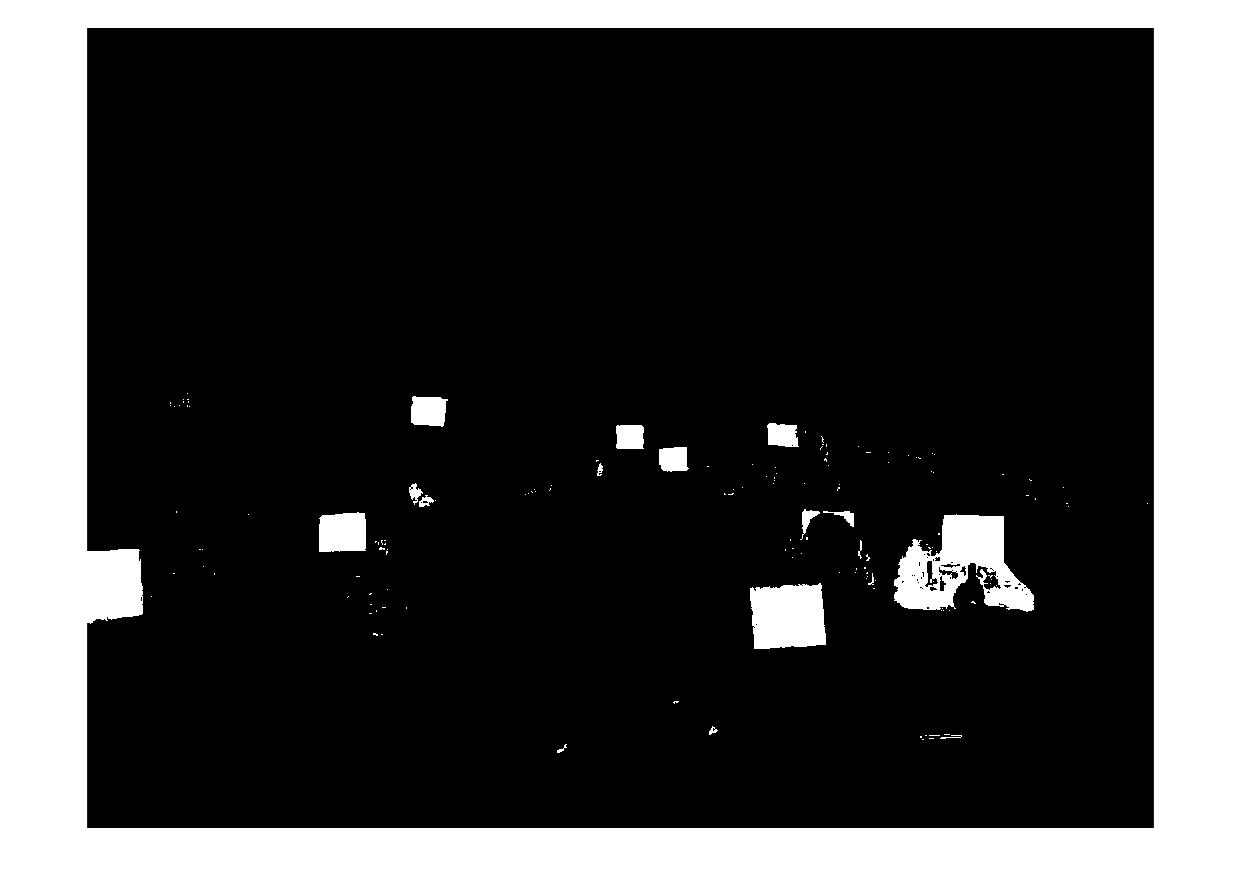
\includegraphics[width=0.45\textwidth]{redmask.jpg}
    \hfill
    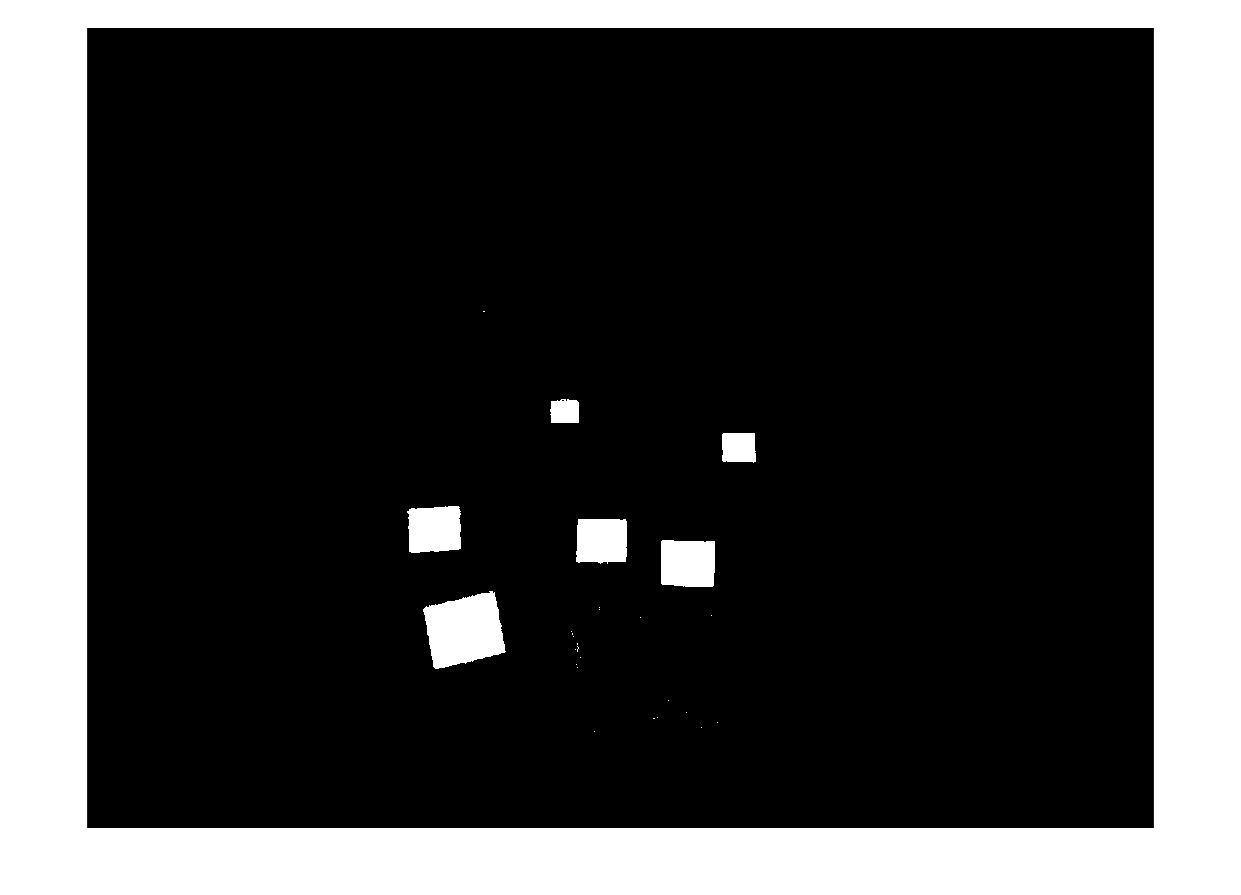
\includegraphics[width=0.45\textwidth]{greenmask.jpg} 
    \caption{a) redMask b) greenMask}
    \label{fig:redMaskgreenMask}
\end{figure}

Vidimo da su sa početne slike izdvojena svi regioni gdje se pojavljuju naši kvadrati.

\subsection{Morfološke operacije}
\lstinputlisting[language=matlab, style=mystyle, linerange={40-43}]{../brojanje_kvadrata_ciz.m}

U obradi slike, matematička morfologija je korištena kao sredstvo za identificiranje i ekstrakciju značajnih deskriptora slike na osnovu osobina oblika unutar slike. \\

Ključno područje primjene morfologije predstavlja segmentacija slike, zajedno sa automatskim brojenjem i inspekcijom. 
Morfološke operacije su također osnovni alati te se kao takvi primarno koriste u binarnim slikama, ali se mogu primjeniti i na sive slike.
 Ove operacije direktno koriste matematičke metode za analizu i promjenu strukture objekta. \\

Ključni operatori su \textit{dilatacija i erozija}. \\

Moguće je sve složenije procedure svesti na dvije pomenute. 
Osvrćući se na sam pojam binarne slike, on je obrađen u prethodnom tekstu. 
Međutim, važno je pomenuti da se binarna slika sastoji od bilo koje grupe povezanih piksela. Tu dolazi do razlike između dvije vrste povezanosti i to 4-povezanost i 8-povezanost. 4-povezanost se temelji na povezanosti piksela koji su u neporednoj horizontalnoj ili vertikalnoj blizini. 
To znači da su povezani samo oni pikseli koji se nalaze uzduž stranica kvadrata, a ne dijagonalno. Pikseli \textbf{(i, j)} su povezani ako postoji neki piksel u njegovom neposrednom okruženju, koji je u istoj boji (npr. bijeli piksel u binarnoj slici), a taj piksel se nalazi u jednoj od sledećih pozicija:
\begin{itemize}
\item (i-1, j) — gornji susjed
\item (i+1, j) — donji susjed
\item (i, j-1) — lijevi susjed
\item (i, j+1) — desni susjed

\end{itemize}
Ovaj tip povezanosti primjenjuje se kada je potrebno razmatrati samo vertikalne i horizontalne susjede za povezivanje piksela. \\

Za 4-povezanost, N4, koristi se city-block ili Manhattan distanca.
8-povezanost se temelji na širem okruženju, gdje su povezani pikseli koji se nalaze u neposrednom susjedstvu, uključujući vertikalne, horizontalne, i dijagonalne susjede. Dakle, osim vertikalnih i horizontalnih piksela, uključeni su i dijagonalni susjedi.\\

Pikseli \textit{ (i, j)} su povezani ako postoji neki piksel u njegovom neposrednom okruženju, koji je u istoj boji, a taj piksel se nalazi u jednoj od sledećih pozicija:
\begin{itemize}
\item (i-1, j) — gornji susjed
\item (i+1, j) — donji susjed
\item (i, j-1) — lijevi susjed
\item (i, j+1) — desni susjed

\item (i-1, j-1) — gornji lijevi dijagonalni susjed
\item (i-1, j+1) — gornji desni dijagonalni susjed
\item (i+1, j-1) — donji lijevi dijagonalni susjed
\item (i+1, j+1) — donji desni dijagonalni susjed

\end{itemize}

Primenjuje se kada je potrebno razmatrati sve susjede, uključujući dijagonalne, za povezivanje piksela.
 Za 8-povezanost, N8, koristi se Chebysheva ili šahovska distanca. \\
Dakle, korišćenje 8-povezanosti može biti korisno kada želimo da prepoznamo objekte koji su "nešto razdvojeni", ali su dijagonalno povezani, dok 4-povezanost može biti korisna kada želimo da analiziramo striktne vertikalne ili horizontalne veze između objekata.
\\ \\
Sljedeći bitan pojam, koji služi objašnjavanju gornjih operacije, jeste strukturni element.\\

 \textbf{Strukturni elementi (SE) }su osnovni alati u morfološkoj obradi slike.
Oni su matrice sa fiksnim oblikom koje se koriste za primjenu različitih morfoloških operacija na binarnim ili grayscale slikama. 
Strukturni element definiše oblik i veličinu regiona u okolini svakog piksela slike, koji se koristi za manipulaciju tim pikselima tokom morfoloških operacija. 
SE mogu imati različite oblike kao što su kružni, kvadratni, pravougaoni, dok njihova veličina zavisi direktno od njihove aplikacije u samom kodu. 
Navedeni pojmovi su ključni pri pristupu eroziji i dilataciji. \\

Najprije, \textbf{erozija} se koristi za smanjenje objekata na slici. Ova operacija omogućava uklanjanje manjih struktura i detalja u slici, kao i smanjenje veličine objekata u binarnoj slici.
Erozija je vrlo korisna u segmentaciji, uklanjanju šuma i prepoznavanju oblika. 
Erozija funkcioniše tako što, za svaki piksel u slici, gleda sve njegove susjedne piksele. 
Ako svi susjedni pikseli koji čine oblik strukturnog elementa imaju vrijednost 1 (odnosno pripadaju objektu), onda centralni piksel ostaje 1. Ako neki od susjednih piksela nije 1, centralni piksel se postavlja na 0, što znači da se objekat smanjuje.

S druge strane, \textbf{dilatacija} se koristi za proširivanje objekata na slici. 
Ova operacija omogućava povećanje veličine objekata u binarnoj slici i povezivanje objekata koji su blizu jedan drugog. 
Dilatacija je suprotnost eroziji, jer proširuje piksele objekta umjesto da ih smanjuje. 
Dilatacija koristi strukturni element (SE) koji se "širi" oko svakog piksela objekta u slici. 
Za svaki piksel u slici, dilatacija postavlja vrijednost 1 u centralni piksel (ako je bar jedan piksel iz strukturnog elementa 1). 
Ako je bar jedan od susjednih piksela 1, centralni piksel postaje 1. 
Dakle, objekat se "proširuje" tako da susjedni pikseli postaju dio objekta. 
\\
Dilatacija i erozija se često koriste zajedno. Na primjer, primjena dilatacije može učiniti objekat većim, dok erozija može ukloniti nepotrebne dijelove objekta.
 Ove operacije zajedno čine osnovu mnogih "otvoreno" i "zatvoreno" morfoloških operacija. \\

\textbf{Otvaranje} je definisano kao morfološka operacija erozije praćena sa dilatacijom sa istim strukturnim elementom. 
Erozija uklanja neke piksela objekta sa ivica regiona objekta, dok dilatacija dodajepiksele objekta. Tako veličina objekta ostaje ista, ali su njegove konture zaglađenije. \\

\textbf{Zatvaranje} je morfološka operacija koja se sastoji od dilatacije praćene erozijom sa istim strukturnim elementom. 
Zatvaranje zaglađuje konture objekata, ali i popunjava uske prekide ili praznine i eliminiše male šupljine, mijenjajući te male regione pozadine u regione objekta.

Gore navedeni kod koristi nekoliko morfoloških operacija za obradu slike u kojoj je detektovana crvena boja, pri čemu je isti pristup urađen i za zelenu boju. 
Morfološke operacije koriste strukturne elemente za manipulaciju oblikom objekata u slici. 
U ovom slučaju, strukturni element je disk, što znači da se koristi diskasti oblik za primjenu operacija.
\\

\texttt{redMask = imerode(redMask, strel('disk', 3));}
\\

Ovdje se primenjuje erozija na \texttt{redMask} koristeći \textbf{diskasti strukturni element} sa poluprečnikom od 3 piksela. 
Ovaj diskasti strukturni element je matrica koja sadrži vrijednosti 1 u obliku diska (poluprečnik 3) i 0 izvan tog diska. 
Erozija će ukloniti piksele sa ivica objekta. 
Zbog ove operacije, objekti u redMask postaju manji, a sitni objekti mogu biti uklonjeni. Ova operacija se radi dva puta uzastopno.\\


\texttt{redMask = imopen(redMask, strel('disk', 10));}\\

U ovoj liniji je primjenjena otvorena operacija. Prvo se smanjuju objekti pomoću erozije, a zatim se proširuju pomoću dilatacije.  
Ovaj postupak služi za uklanjanje sitnih objekata i šupljina u većim objektima, dok istovremeno zadržava osnovnu strukturu objekata. 
Zbog erozije, manji objekti nestaju, dok dilatacija omogućava da preostali objekti ponovo postanu "veći" i sačuvaju osnovni oblik.\\


\texttt{redMask = imdilate(redMask, strel('disk', 10));}\\

Ovom linijom se proširuju preostali objekti u slici koristeći diskasti strukturni element. Ovo može povezati objekte koji su se prethodno razdvojili i može proširiti ivice objekata, čineći ih "većim".
Ovaj niz operacija omogućava precizno filtriranje i obradu binarnih slika, sa ciljem da se izdvoje važni objekti (u ovom slučaju crvena boja) i da se poboljša njihova vidljivost i konture na slici.


\begin{figure}[htbp]
    \centering
    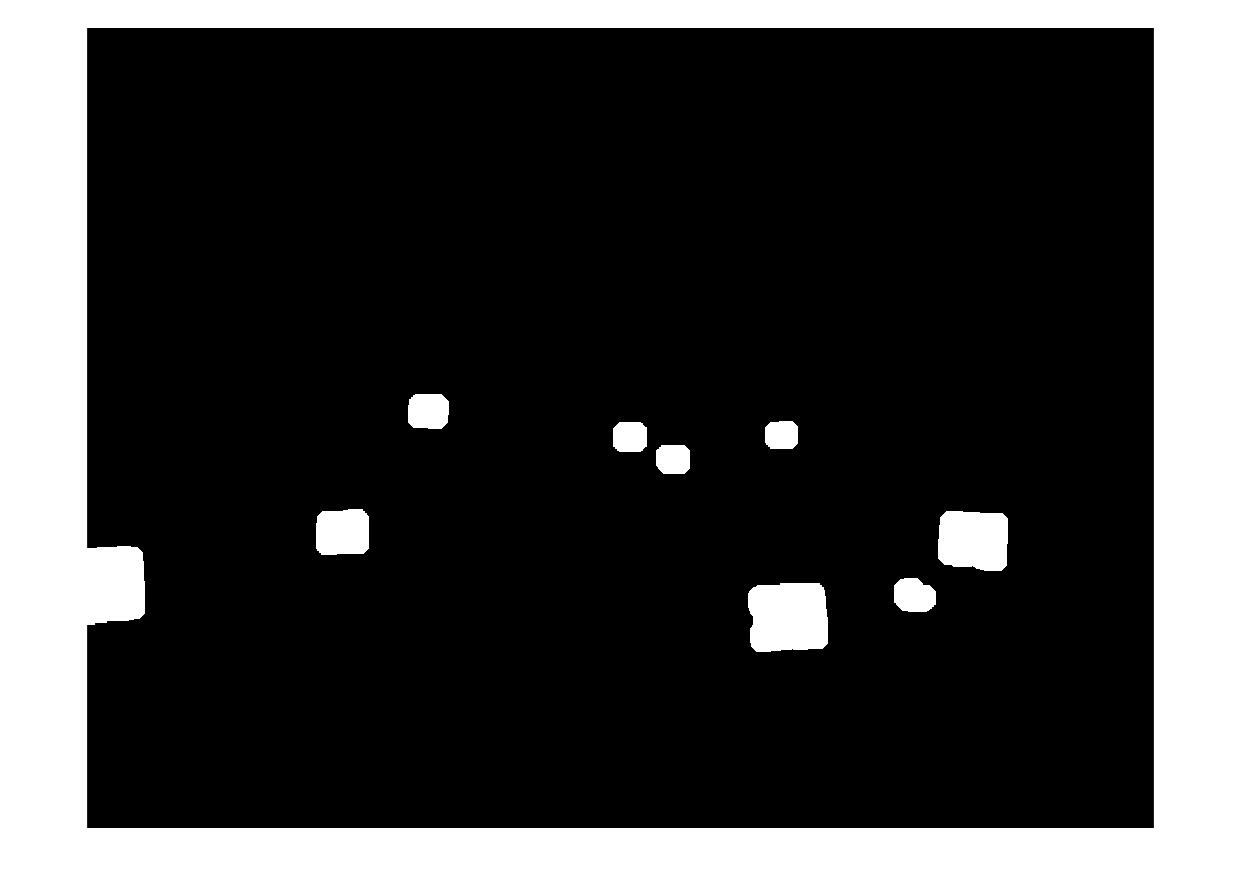
\includegraphics[width=0.49\textwidth]{morphred.jpg}
    \hfill
    
\includegraphics[width=0.49\textwidth]{morphgreen.jpg} 
    \caption{redMask i greeenMask nakon morfoloških operacija}
    \label{fig:redMaskgreenMask}
\end{figure}


\subsection{Boundary}


\lstinputlisting[language=matlab, style=mystyle, linerange={55-56}]{../brojanje_kvadrata_ciz.m}

\subsection{Funkcija brojanje}

Poziv funkcije:

\lstinputlisting[language=matlab, style=mystyle, linerange={73-74}]{../brojanje_kvadrata_ciz.m}

Funkcija:

\lstinputlisting[language=matlab, style=mystyle]{../Funkcija_brojanje.m}
\newpage
Rezultat:

\begin{figure}[h]
    \centering
    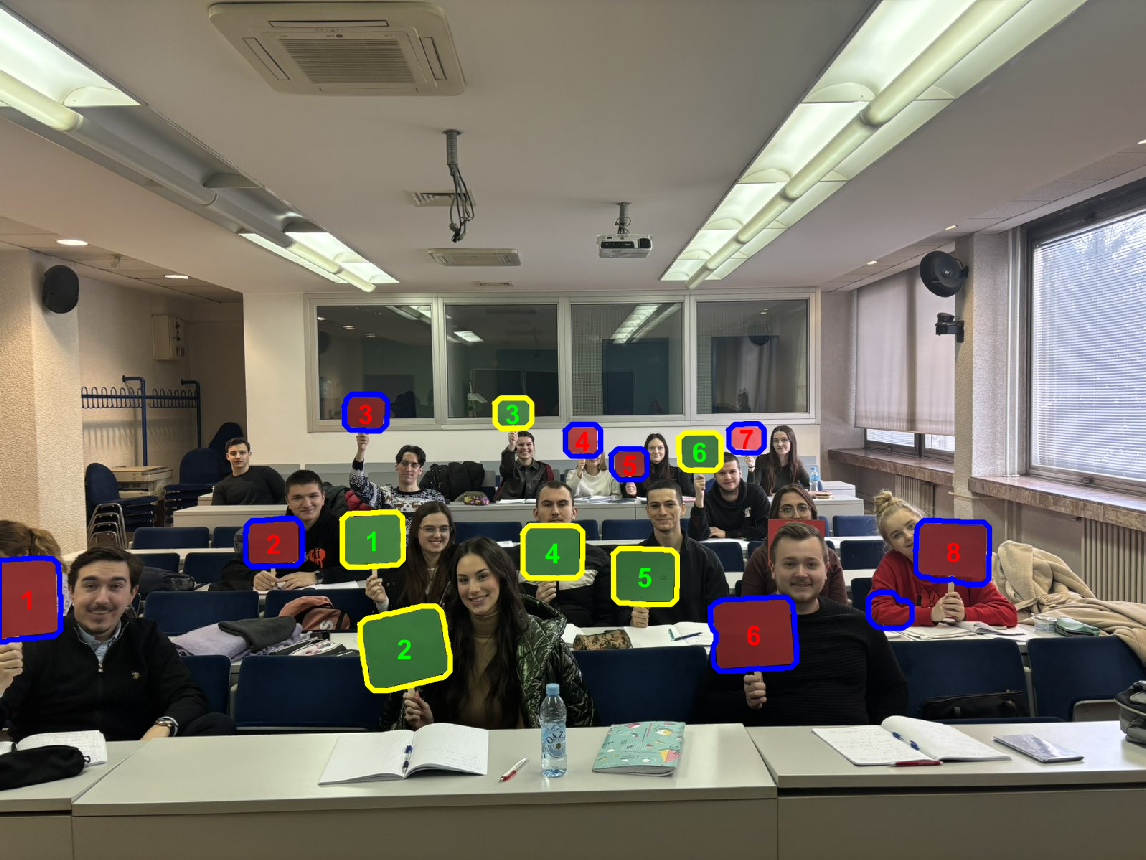
\includegraphics[width=\textwidth]{studenti.png}
    \caption{8 crvenih 6 zelenih}
    \label{fig:example}
\end{figure}
\section{Zaključak:}
\newpage
\section{Izvori:}

\end{document}
